\chapter[Classical Radiative Transfer][Classical Radiative Transfer]{Classical Radiative Transfer} \label{ap:CRT} \allowdisplaybreaks

\section{Emissive Power of a Blackbody}
%
Define the quantity $e_{\lambda}$ as the monochromatic emissive power (with units of \si{\watt\per\square\meter\per\meter}), which gives the flux of energy radiated from a surface at a given wavelength and temperature. Then 
%
\begin{equation}
e(T) = \int_{0}^{\infty} e_{\lambda}(\lambda, T) d\lambda
\end{equation}
%
gives the total energy flux emitted by the surface at a given temperature. Planck's blackbody law gives $e_{\lambda, BB}$, the monochromatic emissive power of a blackbody, as
%
\begin{equation}\label{eq:BlackBody_Power}
    e_{\lambda, BB}(T,\lambda) = \frac{2 \pi h c^{2}}{\lambda^{5}} \frac{1}{\exp{\left( \frac{hc}{\lambda k_{B}T} \right)} -1}
\end{equation}
%
where $h$ is Planck's constant, $c$ is the speed of light in vacuum, $\lambda$ is the wavelength in vacuum, $k_{B}$ is Boltzmann's constant, and $T$ is the thermodynamic temperature. Integrating to get the total emitted power yields
\begin{equation} \label{eq:StefanBoltzmannLaw}
e_{BB}(T) = \int_{0}^{\infty} e_{\lambda, BB}(\lambda, T) d\lambda = \sigma T^{4}
\end{equation}
%
where $\sigma = 2 \pi^{5} k_{B}^{4}/( 15 c^{2} h^{3} )$ is the Stefan-Boltzmann constant. This is the Stefan-Boltzmann law.

\section{Emissivity}
%
Real objects do not emit exactly like blackbodies, so it is useful to benchmark a real object's emission against that of a blackbody. The ratio of a real object's monochromatic emissive power to that of a blackbody is called the object's spectral emissivity, $\epsilon_{\lambda}$. It is given by $\epsilon_{\lambda} = e_{\lambda} / e_{\lambda, BB}$. Another useful quantity is the total emissivity, which gives the ratio of an object's total emitted power to that of a black body, and is given by
%
\begin{equation}
\epsilon = \frac{e(T)}{e_{BB}(T)} = \frac{ \int_{0}^{\infty} e_{\lambda}(T) d\lambda }{ \int_{0}^{\infty} e_{\lambda,BB}(T) d\lambda } = \frac{ \int_{0}^{\infty} \epsilon_{\lambda} e_{\lambda,BB}(T) d\lambda }{ \int_{0}^{\infty} e_{\lambda,BB}(T) d\lambda } = \frac{ \int_{0}^{\infty} \epsilon_{\lambda} e_{\lambda,BB}(T) d\lambda }{\sigma T^{4}}
\end{equation}


\section{View Factor}
%
The view factor, $F_{i \rightarrow  j}$, is the proportion of rays of light that are emitted diffusely (isotropically) from surface $i$ that strike surface $j$. It is given by the double integral
%
\begin{equation}\label{eq:ViewFactor}
	A_{i} F_{i \rightarrow j} = \int_{A_{i}} \int_{A_{j}} \frac{ \cos{\theta_{i}} \cos{\theta_{j}} }{ \pi S^{2} } dA_{i}dA_{j}
\end{equation}
%
where $A$ is the surface area of an object and $\theta$ and $S$ are configuration parameters which are defined in Fig. \ref{fig:ViewFactor}. The view factor has two very important properties: $A_{i} F_{i \rightarrow  j} = A_{j} F_{j \rightarrow i}$ (which becomes readily apparent by swapping instances of $i$ and $j$ in Eq. \ref{eq:ViewFactor}) and $\sum_{j} F_{i \rightarrow  j} = 1$ (which is a mathematical statement that that all emitted rays must go somewhere).

\begin{figure}
\centering
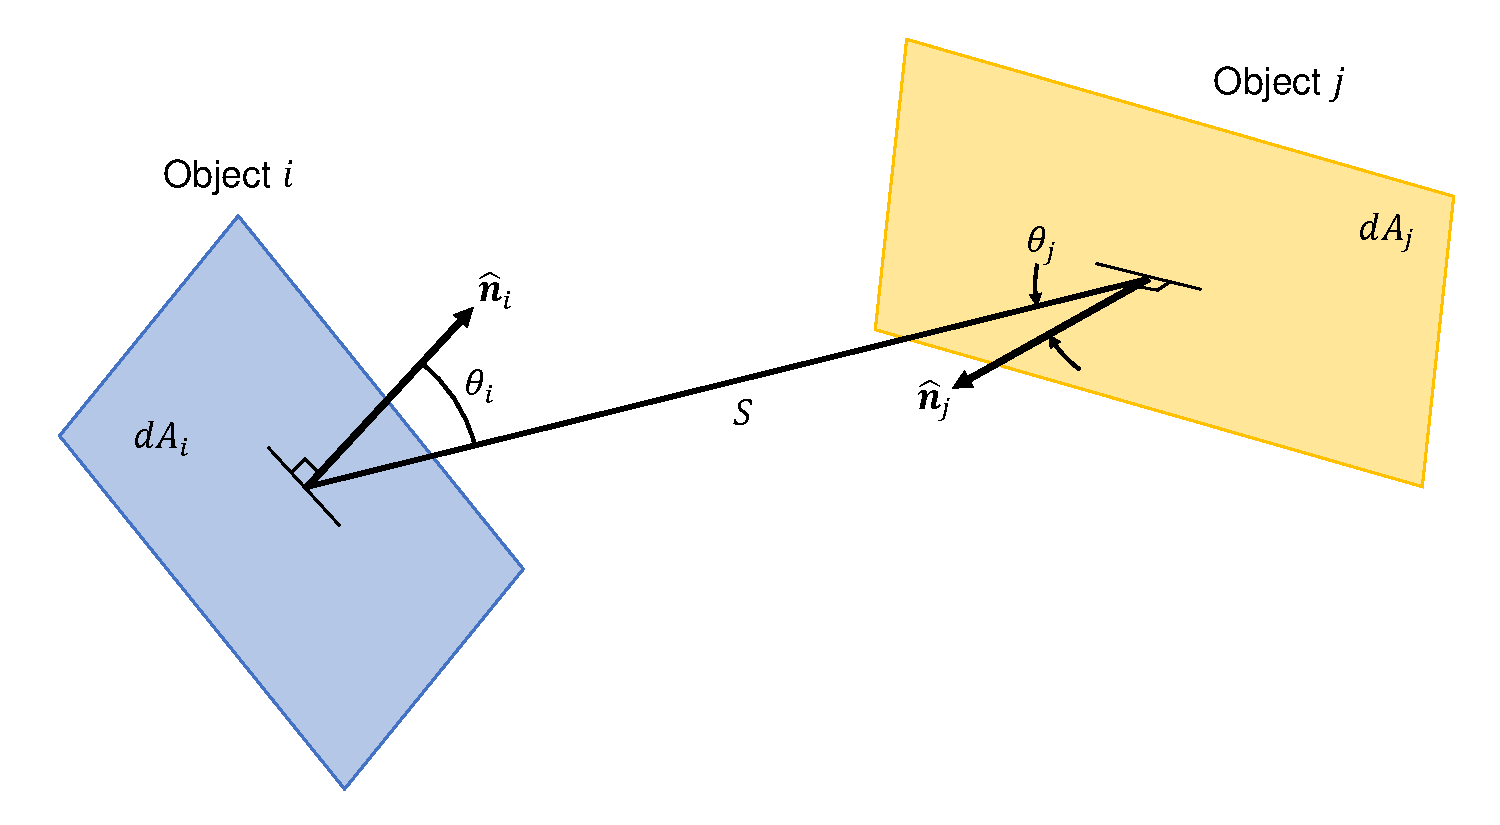
\includegraphics[width=0.8\textwidth]{./Figures/ViewFactor.pdf}
\caption{\label{fig:ViewFactor}Diagram of geometric parameters necessary to compute a view factor.}
\end{figure}


\section{Radiative Heat Transfer}
%
If objects $i$ and $j$ are blackbodies, the total radiative power emitted by object $i$ that strikes object $j$  is given by
%
\begin{equation} \label{eq:RadiatedPower}
Q_{i \rightarrow j, BB} = \sigma T_{i}^{4} A_{i} F_{i \rightarrow j}
\end{equation}

A similar quantity for emission by object $j$ can be obtained by swapping $i$ and $i$ in Eq. \ref{eq:RadiatedPower}. Their net power exchange is
%
\begin{equation} \label{eq:RadiatedPower}
Q_{i \rightarrow j, BB}^{(net)} = Q_{i \rightarrow j, BB} - Q_{j \rightarrow i, BB} = \sigma A_{i} F_{i \rightarrow j} \left( T_{i}^{4} - T_{j}^{4} \right)
\end{equation}

If objects $i$ and $j$ are not blackbodies, then not all radiation which is emitted by object $i$ will be absorbed by object $j$ when it strikes its surface. Instead, some will reflect off object $i$ and potentially be reabsorbed by object $i$, which would not contribute to the net radiative transfer. Accounting for these reflections,
%
\begin{align*}
    Q_{i \rightarrow j} &= \left( \epsilon_{i} \sigma T_{i}^{4} A_{i} \right) F_{i \rightarrow j} \alpha_{j} \\
    &+ \left( \epsilon_{i} \sigma T_{i}^{4} A_{i} \right) F_{i \rightarrow j} \left( \rho_{j} F_{j \rightarrow i} \rho_{i} F_{i \rightarrow j} \right) \alpha_{j} \\
    &+ \left( \epsilon_{i} \sigma T_{i}^{4} A_{i} \right) F_{i \rightarrow j} \left( \rho_{j} F_{j \rightarrow i} \rho_{i} F_{i \rightarrow j} \rho_{j} F_{j \rightarrow i} \rho_{i} F_{i \rightarrow j} \right) \alpha_{j} \\
    &+ ... \\
    &= \left( \epsilon_{i} \sigma T_{i}^{4} A_{i} \right) F_{i \rightarrow j} \alpha_{j} \sum_{n=0}^{\infty} \left( \rho_{j} F_{j \rightarrow i} \rho_{i} F_{i \rightarrow j}\right)^{n} \\
    &= \frac{\epsilon_{i} \alpha_{j} \sigma T_{i}^{4} A_{i} F_{i \rightarrow j}}{1- \rho_{i} \rho_{j} F_{i \rightarrow j} F_{j \rightarrow i} } \\
    &= \frac{\epsilon_{i} \epsilon_{j} \sigma T_{i}^{4} A_{i} F_{i \rightarrow j}}{1- (1-\epsilon_{i}) (1-\epsilon_{j}) F_{i \rightarrow j} F_{j \rightarrow i} }
\end{align*}
%
and
%
\begin{equation}
    Q_{i \rightarrow j}^{(net)} = \left( \frac{\epsilon_{i} \epsilon_{j} }{1- (1-\epsilon_{i}) (1-\epsilon_{j}) F_{i \rightarrow j} F_{i \rightarrow j} } \right) Q_{i \rightarrow j, BB}^{(net)}
\end{equation}
%
where $\alpha = \epsilon$ is the absorptivity and $\rho = 1 - \epsilon$ is the reflectivity. 